% =====================================================================
%  P290_poster.tex  —  A0 portrait conference poster
%  Helical Attractors on Contact 3-Manifolds
%  XII Bienal da SBM · UFRN, Natal-RN · P290 · quinta 06/08/2026, 16:00
%  Build: pdflatex P290_poster.tex   (needs fig_*.pdf + the two logos)
% =====================================================================
\documentclass[final]{article}
\usepackage[T1]{fontenc}
\usepackage[utf8]{inputenc}
\usepackage{lmodern}
\usepackage{amsmath,amssymb}
\usepackage{graphicx}
\usepackage[table]{xcolor}
\usepackage{multicol}
\usepackage{booktabs}
\usepackage{tikz}
\usepackage[paperwidth=841mm,paperheight=1189mm,margin=38mm,top=34mm,bottom=30mm]{geometry}
\usepackage{microtype}
\pagestyle{empty}
\setlength{\parindent}{0pt}
\setlength{\columnsep}{26mm}
\setlength{\columnseprule}{0pt}

\definecolor{ink}{RGB}{28,28,36}
\definecolor{navy}{RGB}{28,90,140}
\definecolor{gold}{RGB}{200,137,31}
\definecolor{brick}{RGB}{176,48,48}
\definecolor{paper}{RGB}{252,251,248}
\definecolor{band}{RGB}{242,240,233}
\definecolor{rule}{RGB}{200,198,190}

\pagecolor{paper}
\color{ink}

% ---- scaled type ----
\newcommand{\Body}{\fontsize{27}{36}\selectfont}
\newcommand{\Small}{\fontsize{22}{29}\selectfont}
\newcommand{\Head}[1]{%
  \vspace{7mm}{\fontsize{34}{40}\selectfont\bfseries\color{navy}#1}\\[-1mm]
  {\color{gold}\rule{\linewidth}{2.2pt}}\\[5mm]}

% ---- boxes ----
\newcommand{\keybox}[2]{%
  \begin{tikzpicture}
    \node[fill=band,draw=gold,line width=2pt,inner sep=8mm,text width=\dimexpr\linewidth-18mm\relax,
          rounded corners=2pt] {%
      \begin{minipage}{\dimexpr\linewidth-18mm\relax}
        {\fontsize{23}{28}\selectfont\bfseries\color{gold}\MakeUppercase{#1}}\\[4mm]
        \Body #2
      \end{minipage}};
  \end{tikzpicture}\\[6mm]}

\begin{document}
\Body

% =====================================================================
%  HEADER
% =====================================================================
\begin{minipage}[c]{0.13\linewidth}
  
\includegraphics[width=\linewidth]{LogoXIIBienal.png}
\end{minipage}\hfill
\begin{minipage}[c]{0.66\linewidth}\centering
  {\fontsize{62}{72}\selectfont\bfseries Helical Attractors on\\ Contact 3-Manifolds}\\[6mm]
  {\fontsize{32}{38}\selectfont\itshape Atratores Helicoidais em Variedades de Contato}\\[8mm]
  {\fontsize{30}{36}\selectfont\bfseries Pablo Nogueira Grossi}\\[3mm]
  {\fontsize{24}{30}\selectfont G6 LLC \;\textbullet\; Newark, NJ \;\textbullet\; \texttt{pg6llc@gmail.com}}\\[2mm]
  {\fontsize{22}{28}\selectfont ORCID 0009-0000-6496-2186}
\end{minipage}\hfill
\begin{minipage}[c]{0.15\linewidth}
  
\includegraphics[width=\linewidth]{UFRN2.png}
\end{minipage}

\vspace{7mm}
{\color{navy}\rule{\linewidth}{4pt}}\\[3mm]
{\fontsize{24}{30}\selectfont\bfseries P290}\;\textbullet\;
{\fontsize{24}{30}\selectfont XII Bienal da SBM · UFRN, Natal-RN · quinta 06/08/2026, 16:00–17:00 ·
Saguão dos Anfiteatros do CCET}\\[2mm]
{\color{navy}\rule{\linewidth}{4pt}}

\vspace{10mm}

% =====================================================================
\begin{multicols}{3}

% ------------------------------ COL 1
\Head{The system}
On the contact 3-manifold $(\mathbb{R}^3,\alpha)$ with
$\alpha = dz - r^2\,d\theta$ and Reeb field $R=\partial_z$, write a state as
$(r,\theta,z)$. The system $\mathrm{dm}^3$ is
\vspace{3mm}

{\fontsize{24}{34}\selectfont
$\dot r = r(1-r^2) + \varepsilon(r-1)e^{-z}$\\[2mm]
$\dot\theta = 1$\\[2mm]
$\dot z = r^2 - \varepsilon(r-1)^2e^{-z}$
}
\vspace{4mm}

with $\varepsilon = 2$. The cylinder $\Gamma=\{r=1\}$ is invariant and carries the helical flow
$\dot\theta=\dot z=1$ — a lift of the Reeb orbit.

\vspace{3mm}
\textbf{The question: does $\Gamma$ attract?}

\Head{Main theorem}
\keybox{Theorem 2.1}{%
For initial data with $|r(0)-1| < 1/3$ and $z(0)\ge\log 2$, the solution exists for all $t\ge 0$ and
\[|r(t)-1| \;\le\; C\,|r(0)-1|\,e^{-2t},\]
so every such orbit converges exponentially to $\Gamma$ at the rate $\mu=-2$ — the Jacobian
eigenvalue of the radial part at $r=1$.}

\Small
\textit{Proof.} Gronwall. Squaring the radial equation gives
$\tfrac12\tfrac{d}{dt}u^2 \le -2u^2-3u^3-u^4+\varepsilon u^2e^{-z}$ with $u=r-1$; the hypothesis on
$z(0)$ forces the last term to be dominated on the relevant window. $\square$
\Body

\vspace{5mm}
\begin{center}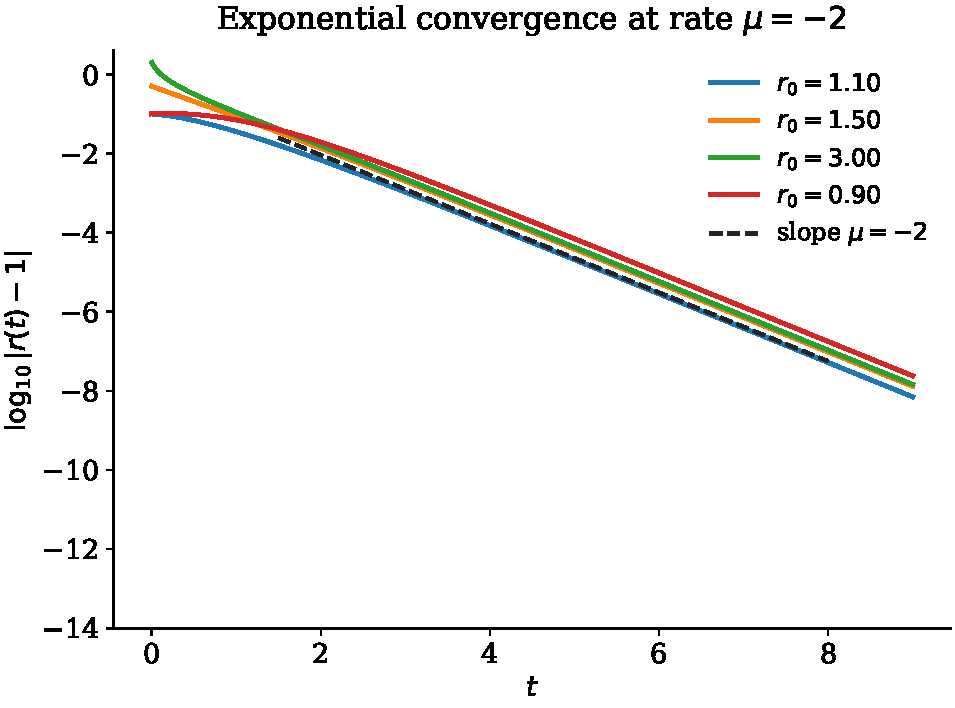
\includegraphics[width=\linewidth]{fig_decay.pdf}\end{center}

\columnbreak
% ------------------------------ COL 2
\Head{Basin asymmetry}
Numerically the basin is \emph{not} symmetric about $\Gamma$. Outward, every tested initial condition
converges. Inward, orbits collapse — $r\to 0$, $z\to-\infty$ in finite time.

\vspace{4mm}
\begin{center}
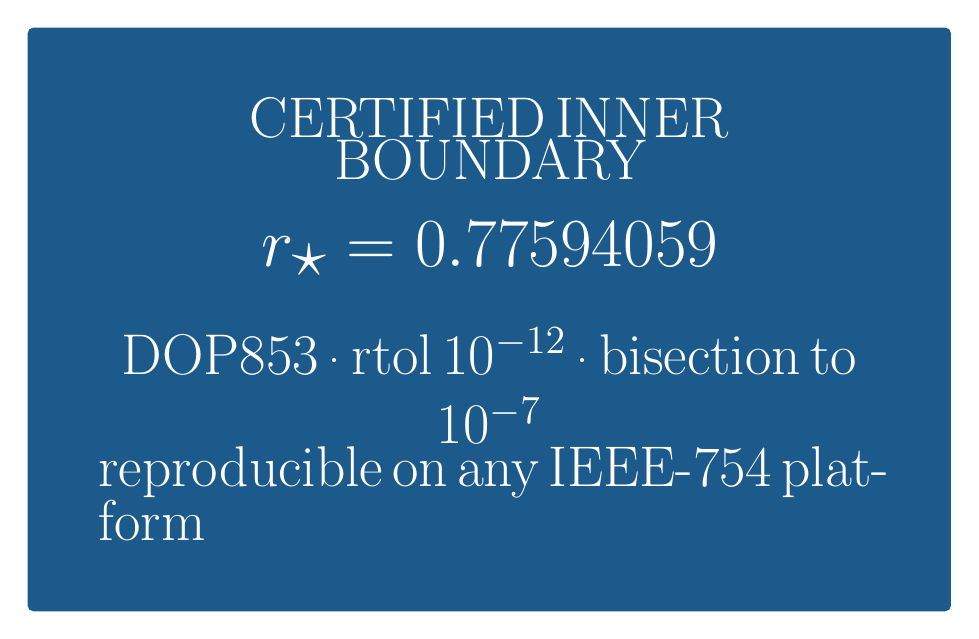
\begin{tikzpicture}
\node[fill=navy,inner sep=9mm,text width=\dimexpr\linewidth-22mm\relax,rounded corners=2pt]{%
  \centering\color{white}
  {\fontsize{22}{26}\selectfont CERTIFIED INNER BOUNDARY}\\[5mm]
  {\fontsize{56}{60}\selectfont\bfseries $r_\star = 0.77594059$}\\[5mm]
  {\fontsize{20}{25}\selectfont DOP853 · rtol $10^{-12}$ · bisection to $10^{-7}$\\
  reproducible on any IEEE-754 platform}};
\end{tikzpicture}
\end{center}
\vspace{5mm}

Since $r_\star > 2/3$, the interval $(2/3,\,r_\star)$ holds initial data \emph{inside} the Gronwall
ball that nevertheless escape. This does not contradict Theorem 2.1 — the second hypothesis
$z(0)\ge\log 2$ is exactly what excludes them.

\vspace{4mm}
\begin{center}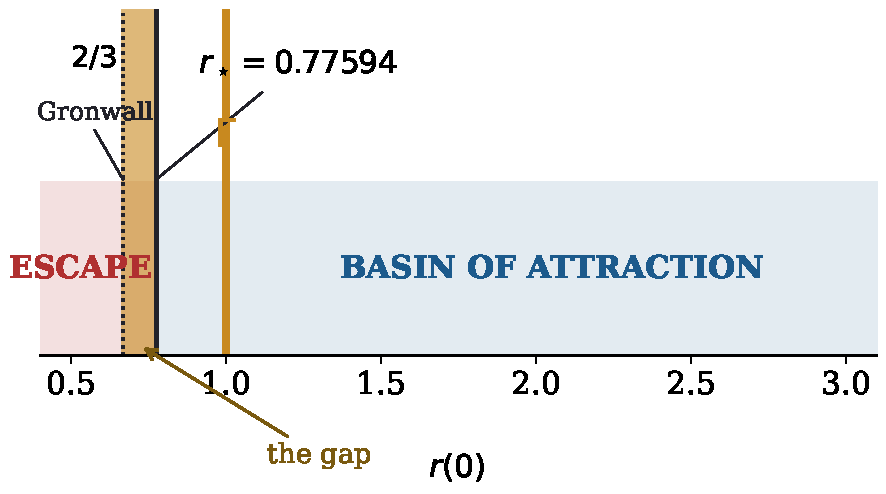
\includegraphics[width=\linewidth]{fig_basin.pdf}\end{center}
\vspace{3mm}
\begin{center}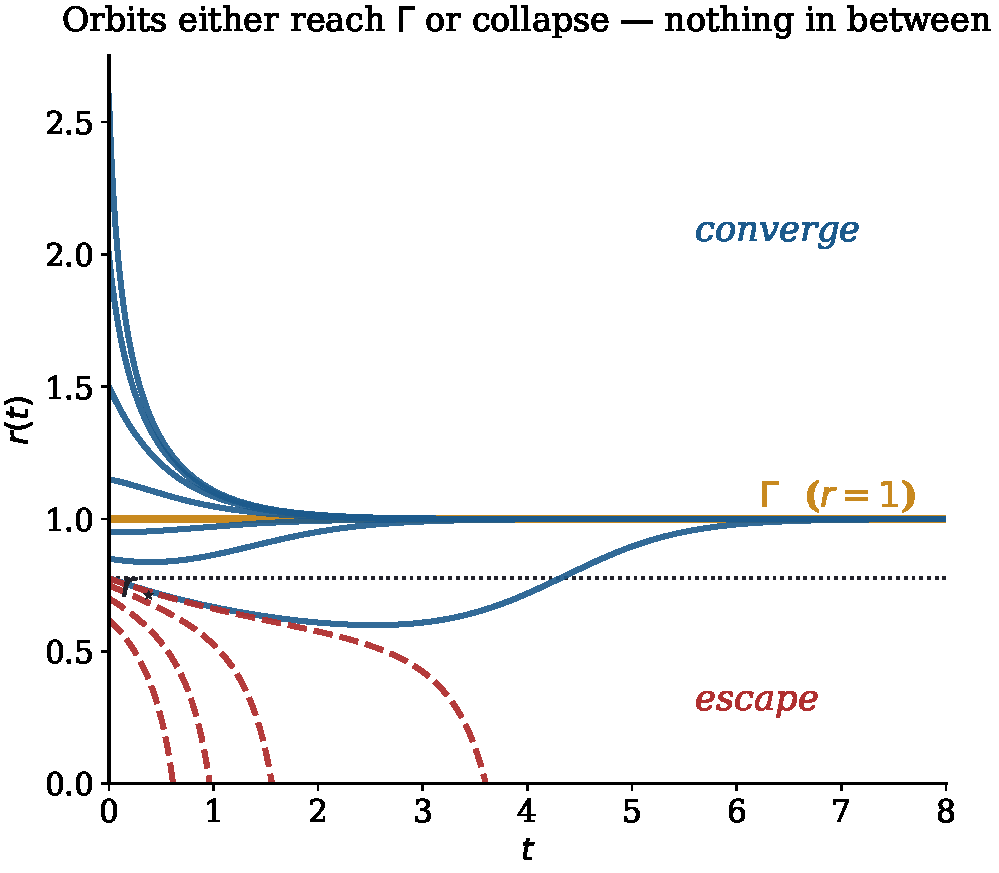
\includegraphics[width=\linewidth]{fig_phase.pdf}\end{center}

\columnbreak
% ------------------------------ COL 3
\Head{A scaling law}
The pair $(\varepsilon,z(0))$ enters the dynamics \emph{only} through
\[\lambda \;=\; \varepsilon\,e^{-z(0)},\]
since $\varepsilon$ and $e^{-z}$ never occur apart. Every basin quantity is a function of $\lambda$
alone — verified to $10^{-12}$ across independent $(\varepsilon,z_0)$ pairs.

\vspace{4mm}
\begin{center}
{\fontsize{25}{33}\selectfont
\begin{tabular}{@{}rl@{}}
\toprule
$\lambda$ & $r_\star$\\
\midrule
$0.5$ & $0.377975$\\
$1.0$ & $\mathbf{0.572235}$ \;{\footnotesize($z_0=\log 2$)}\\
$2.0$ & $\mathbf{0.775941}$ \;{\footnotesize($z_0=0$)}\\
$3.0$ & $0.878915$\\
\bottomrule
\end{tabular}}
\end{center}
\vspace{4mm}

\begin{center}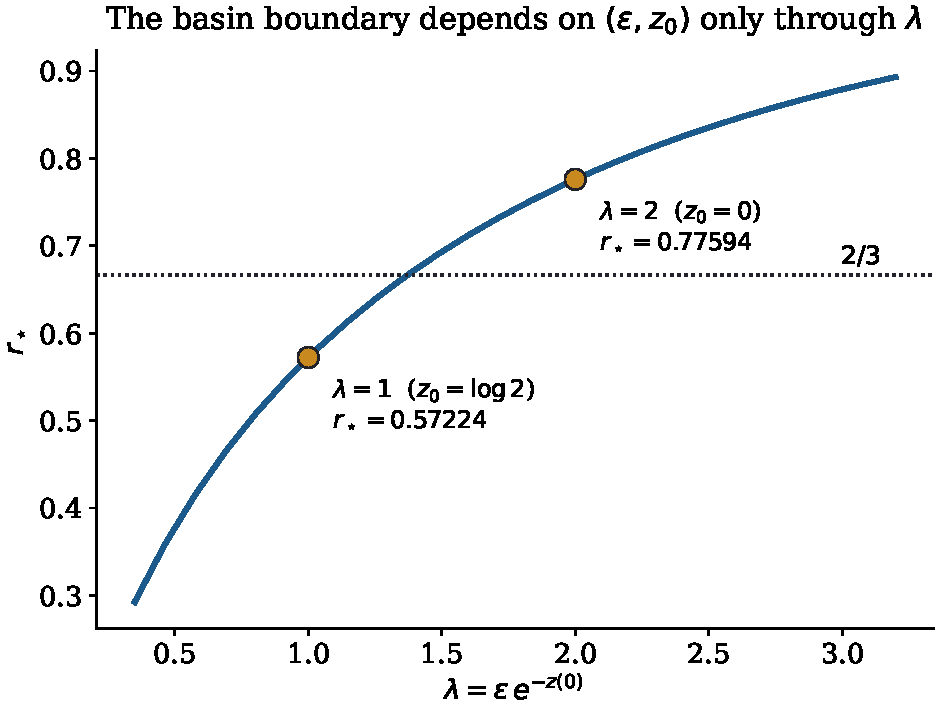
\includegraphics[width=\linewidth]{fig_lambda.pdf}\end{center}
\vspace{3mm}

At $\lambda=1$ one finds $r_\star < 2/3$: the Gronwall ball sits strictly inside the basin.
\textbf{The hypothesis $z(0)\ge\log 2$ is necessary, not cosmetic.}

\Head{Contact geometry}
The asymmetry $r_\star \ne 2-r_\star$ is diagnostic. It is the fingerprint of the term
$\varepsilon(r-1)^2e^{-z}$ in $\dot z$, which is not symmetric under $u\mapsto -u$ because it couples
to the \emph{non-integrable} direction of $\alpha$. A symmetric basin would mean the attractor
reduces to a 2D problem transverse to $R$; the observed asymmetry says the full 3-manifold contact
structure is essential.

\Head{Status of claims}
{\fontsize{25}{33}\selectfont
\begin{tabular}{@{}p{0.60\linewidth}l@{}}
\toprule
Claim & Status\\
\midrule
$\Gamma$ invariant, $\mu=-2$ & proved\\
Scaling law in $\lambda$ & proved\\
$r_\star = 0.77594059$ & certified numerically\\
Closed form for $r_\star$ & \textbf{open}\\
Lipschitz bound (AXLE \#12) & \textbf{open}\\
\bottomrule
\end{tabular}}
\vspace{5mm}

\Small
\textbf{Reproduce:} \texttt{certify\_rstar.py} — DOP853, deterministic bisection, MIT.\\[2mm]
\textbf{Livro vivo (B3 · Vol.\,III):} \texttt{totogt.github.io/geometry}\\[2mm]
\textbf{Capítulo 10 (Vol.\,IV):} \texttt{totogt.github.io/GTCT}\\[2mm]
\textbf{Formalização:} \texttt{github.com/TOTOGT/AXLE}

\end{multicols}

\vfill
{\color{gold}\rule{\linewidth}{3pt}}\\[7mm]
{\fontsize{34}{40}\selectfont\bfseries\color{navy}What is new here}\\[6mm]
\begin{minipage}[t]{0.305\linewidth}
  {\fontsize{26}{33}\selectfont\bfseries\color{gold}1. The scaling law}\\[3mm]
  {\fontsize{24}{31}\selectfont $(\varepsilon,z_0)$ collapse to the single parameter
  $\lambda = \varepsilon e^{-z_0}$. One curve $r_\star(\lambda)$ replaces a two-parameter family.}
\end{minipage}\hfill
\begin{minipage}[t]{0.305\linewidth}
  {\fontsize{26}{33}\selectfont\bfseries\color{gold}2. The hypothesis earns its place}\\[3mm]
  {\fontsize{24}{31}\selectfont $z(0)\ge\log 2$ is what pulls $r_\star$ below $2/3$. Drop it and the
  Gronwall ball provably contains escaping orbits.}
\end{minipage}\hfill
\begin{minipage}[t]{0.305\linewidth}
  {\fontsize{26}{33}\selectfont\bfseries\color{gold}3. A number you can check}\\[3mm]
  {\fontsize{24}{31}\selectfont $r_\star$ to eight figures, by deterministic bisection, from a script
  that runs in seconds on any machine.}
\end{minipage}

\vspace{9mm}
{\color{rule}\rule{\linewidth}{1.5pt}}\\[3mm]
{\Small\color{ink!70}
Submissões companheiras: \textbf{EXP13} Cimática com Máquinas (Saguão do CETECH, todos os dias)
\;\textbullet\; \textbf{MC48} Minicurso (terça 04/08, E1LAB)
\;\textbullet\; \textbf{CO144} O Princípio do Cajueiro (quarta 05/08, F6)
\;\textbullet\; \textbf{OF53} A Escada de Recorrência (sexta 07/08, H3)
\hfill \copyright\ 2026 Pablo N. Grossi / G6 LLC \;\textbullet\; CC BY 4.0}

\end{document}
